\documentclass[12pt]{article}
\usepackage{graphicx}
\usepackage[margin=1in]{geometry}
\usepackage{indentfirst}
\usepackage{marvosym}

\begin{document}
\section*{Open Source Project}
\subsection*{Steven Rosendahl}

I began this semester with a few open source projects of my own that I've been maintaining. I had had some open source experience before; my capstone project is completely open sourced as well as a repository full of work I've done throughout my college career. Much of the open source work I've done, however, has not been collaborative. At the beginning of the semester, we read over \textit{The Mythical Man Month} which outlined various open source ideas. One of the ideas perpetuated by the author is that open source projects fall under Brook's Law, which states adding more manpower to a project delays the ultimate outcome of the project. In the open source world, however, this phenomenon seems to be absent. The project that we worked on, Habitica, is a prime example of an application making great strides towards completion while having hundreds of contributors. One of the reasons that open source projects grow so quickly towards their goals might actually be due to the lack of communication. Large groups having to communicate often leads to miscommunication; additionally, it takes a lot of time to meet, talk about what needs to be done, and ultimately get around to doing it.\\

One of my least favorite things we did this semester was using Angular.js. I've never been a fan of JavaScript in the first place. Not ever knowing what type of Object you have as well as creating Objects on the fly with no schema makes the process of debugging and contributing very difficult. I also dislike frameworks/languages that force you into a certain design pattern; this is one of the reasons I've never been big into iOS programming. With so many JavaScript frameworks out there, Angular.js is a small fish in a big pond. Python was easier to use due to its structure over JavaScript, but much of the open source world is stuck in Python 2.7 whereas the standard is slowly becoming Python 3. This is a little forgivable, since the tools to convert back and forth between the versions are virtually non-existent. This is definitely a problem that could be fixed by the open source world, but it doesn't appear to be a major focus of the majority of projects, especially the scientific ones for which Python is best known. This behavior seems to appeal to the idea that we shouldn't fix what isn't broken, and being a major version number behind doesn't qualify a project as broken, so it is understandable why many large open source projects are not focusing on migration to Python 3.\\

Midway through the semester, my Apple laptop died, so I was forced to buy a new laptop. Since the newest models of MacBook Pros have only PCIe SSD's in them, I went with a Windows machine; since I don't care for windows, I decided to install Linux; since I was in the middle of the semester and didn't have the time to configure a version like Arch, I decided to install Ubuntu. I've noticed subtle bugs within the Ubuntu distribution that I have, such as the Dock getting stuck and the system not always obeying the Super key. I've been considering looking into the Ubuntu source to see if these issues are fixable by someone with my experience. Linux overall is an incredible example of open source in its prime. The idea that an entire operating system can be driven by an open source community is extraordinary. The main reason that I haven't looked into the source of Ubuntu or Linux is that I wouldn't have anywhere to test my changes and the source is not in a neat place such as Github (the kernal is on Github, but I'm nowhere near experienced enough to mess with it). The Linux operating system is not very different from OS X, so making the switch was not too hard. Originally, I wanted to use a fork of Ubuntu called Elementary OS. The user interface of Elementary OS is very close to that of OS X; ultimately I was not able to make it past the installation onto my computer.\\

About midway through the semester, I encountered a problem with an application that I was writing for my job. The issue involved an \texttt{SSLException} that was being thrown by versions of Android greater than 6.0. In my search for the answer to why this was happening, I came across the open Android project, which is the open source code for the Android operating system. I knew my issue was arising from Android's native implementation of \texttt{okhttp}, so I spent a while trying to pinpoint my error. I was able to narrow it down to something happening in the handshake, but I couldn't go any further since the stack trace given by LogCat was not specific enough to tell me exactly what step in the handshake process was causing an error. After talking with Dr. Koehl, he recommended that I look into the server logs for the particular server that was hosting the data I needed. When I went to our server manager, he noted that the server was rejecting the certificate that my phone was using to connect; his best suggestion was to look into the source code of the program that was running on the server. He directed me to the appropriate repository, and I began looking through to see if I could find anything about certificate validation and why it would be rejecting the requests made from Android 7.0. Ultimately, I was not able to solve this issue (it's still ongoing). Both the Android OS and the code for the server are open source, so it may be possible that others in the community will be able to fix this issue.\\

Habitica was a very large project; I had never dealt with a project on the magnitude of it before. The first step was to get Habitica installed. Since my computer had just recently been setup with Ubuntu and I'm not a JavaScript developer, I had to install Node.js, Bower, and all of the dependencies. The developer's wiki helped marginally, but I was able to get around many of my troubles by performing the installations essentially backwards. This all had to be run under \texttt{sudo}, since Ubuntu is sensitive to touching anything above the \texttt{{\raise.17ex\hbox{$\scriptstyle\sim$}}/} directory. Others in my group found it a little more difficult and had to resort to using Vagrant/Docker to get things up and running since \texttt{npm} wouldn't play nicely. It was hard to find a bug that I though I could easily fix, much less actually fix it. The first few bugs we looked at involved documenting the Habitica API. Unfortunately, this was near impossible without having used Habitica extensively \textbf{and} having knowledge of the public APIs that were provided. We abandoned that idea an moved on to try and fix an issue with notification not appearing on certain critical hits. I began to look extensively into this issue, but I could not find the place in code where notifications were fired for critical hits. We posted in the developer's chat on Habitica's website, but their suggestions did not help very much. Finally, we found another issue which Matthew promptly claimed. The issue we ultimately settled on involved problems with notifications when purchasing gems.
\begin{quote}
    If you set your language to some of the non-English languages and then go to the Market to buy a gem with gold, you receive two notifications for \texttt{+1 gem}, one in your chosen language and then after a short delay, another one in English:
    \begin{center}
        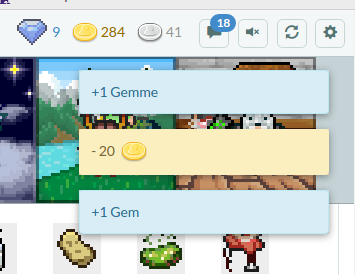
\includegraphics[scale=0.4]{issue}
    \end{center}
    I've tested a few languages and it happens with only those that have a translation for the \texttt{plusOneGem} text that is different than the English version. For example, it happens with German and French, but not with \texttt{en\_GB}, \texttt{en\MVAt pirate}, or \texttt{zh\_TW} all of which still use the default text: \texttt{"plusOneGem": "+1 Gem"}
\end{quote}
To fix this bug we had to first reproduce it. In the local build for Habitica, there was already a button that would grant the user 10 gems, so I managed to wire it to make a purchase without authentication. The goal was to have the notification fire. Once we reproduced the bug, we needed to locate the place where the notification was being fired twice; it turned out to be in the \texttt{userServices.js} file. The way that Habitica determined whether or not a notification had fired was to compare the contents of the notification that should have fired to the contents of the notification that was being created. If they were the same string value, then the program would not create and fire the second notification; if they were different, however, then the second notification would fire. This was a problem only in languages that had translations for the word \textit{Gem} within Habitica. Since, for example, the French word \textit{Gemme} is not the same as the English translation \textit{Gem}, the notification fired again with \textit{Gem}. To fix this, we simply added a boolean that checked whether or not a notification had already been fired. If it had, then we wouldn't fire the second one; otherwise we would. This appears to have fixed the problem; the only thing left to do now is test that the problem is truly fixed. It might be the case that the second check to see if a notification was fired is necessary; as such, there may be another issue that arises by just ignoring it.\\

Overall, I think open source projects are one of the greatest developments in software engineering. Being able to root though code yourself and fix your own issues is truly a homage to the idea that \textit{if I don't do it, nobody will}. I've come across a lot of bugs in a lot of places, such as wrestling with a seemingly impossible \texttt{SSLException} in Android to the minor annoyance of broken syntax highlighting in Github's Atom with \LaTeX. The open source community is so influential that many companies such as Microsoft, Apple, and Google support and encourage the use and creation of open source software within their own company. Even if I don't have the skills to fix the problem (or the want to fix the problem), chances are someone out there does. That is the true beauty of open source.
\end{document}
